\section{Methodology}
We treat each consumer-item as an individual object and generate weekly time series based on historical transaction for 
each object. The target value at each time step (week) takes a binary input, 1/0 (purchased/not purchased).
We adopted walk forward Validation strategy for model testing and generalization. We split the data into 4 parts
based on the time series. The last 3 time steps for each of the Time series was used as Validation (hyperparameter Optimization),
Test1 (Stacked Generalization) and Test2 (Reporting Accuracy metric) respectively, and the remaining data was used for training.
We then generate various types of features including datetime related, label encoded and target encoded 
within and across objects. Below are the feature groups with the type of features within each group:
\begin{itemize}
\item {\bf Datetime:} Transactional metrics at various temporal cuts including week, month and quarter. 
Fourier and Taylor functions to capture seasonality and trends.
\item {\bf Consumer Profile:} Total number of orders by the user, Number of distinct items ordered by the user
Time since first order by the shopper, Time since last order by the shopper, Averge time gap between orders
Reorder rate of the user, Reorder frequency of the user, Time of the day user visits, Specific item ordered by user in the past
Order size based features, Orders with no previously reordered item.
\item {\bf Item Profile:} Time since first order for the merchandise, Time since last order for the merchandise
Averge time gap between orders, Reorder rate of the item, Reorder frequency of the item
Number of co-occuring items with this item, Item's average position in the cart, Statistics around order streak for this item
Item's total number of orders, Number of distinct users, Number of users buying it as one shot item.
\item {\bf Consumer-Item Profile:} Time since first order for each combination, Time since last order for each combination
Averge time gap between orders, Reorder rate of the combination, Reorder frequency of the combination, 
Streak -user purchased the item in a row, Average position in the cart, Co-occurance Statistics
Replacement items, Total number of orders for the combination, If user already ordered the item today.
\end{itemize}
The model we needed to build, thus, should learn to identify similarly behaving time series across latent
parameters, and take into account consumer and item variations in comparing the time series. A row in time series 
is represented by

  \begin{equation}
    \begin{array}{l}
      y\textsubscript{cit}  = f(i\textsubscript{t}, c\textsubscript{t},..,c\textsubscript{t-n}, ic\textsubscript{t}
      ,..,ic\textsubscript{t-n}, d\textsubscript{t},..,d\textsubscript{t-n})
    \end{array}
    \label{eqn:fx}
  \end{equation}

where y\textsubscript{cit} is sales for consumer 'c' item ’i’ at time ’t’. 
i\textsubscript{t} is attribute of the item ’i’ like category, department, brand, color, size, etc. 
c\textsubscript{t} is attribute of the consumer 'c' like age, sex and transactional attributes. 
ic\textsubscript{t} is transactional attributes of the consumer 'c'  towards item 'i'. 
d\textsubscript{t} is derived from datetime to capture trend and seasonality. 
Finally, n is the number of time lags.

\subsection{Accuracy Measure}
Since we are solving Binary classification problem, Binary Cross-Entropy/Log Loss [~\ref{eqn:logloss}] seemed most logical loss function 
for training all our models. Also, the same metric was used during stacking to generate final probabilities for 
F1-Maximization. But, we used F1-Score [~\ref{eqn:F1}] values for reporting accuracy as we wanted to maintain a good balance between
Recall and Precision.

  \begin{equation}
      \begin{array}{l}
        H\textsubscript{p} = - \frac{1}{N}$$\sum_{i=1}^{N}y\textsubscript{i}.log(p(y\textsubscript{i}))+
        (1- y\textsubscript{i}).log(1-p(y\textsubscript{i}))
      \end{array}
    \label{eqn:logloss}
  \end{equation}
where y is the label and p(y) is the predicted probability.
Precision refers to the ratio of number of predicted items actually purchased from the predicted items
  \begin{equation}
      \begin{array}{l}
        Precision = \frac{TP} {TP + FP}
      \end{array}
    \label{eqn:Precision}
  \end{equation}
where TP refers to True Positive and FP refers to False Positive.
Recall refers to the ratio of predicted items actually purchased from the items in the actual basket. 
  \begin{equation}
      \begin{array}{l}
        Recall = \frac{TP} {TP + FN}
        \end{array}
    \label{eqn:Recall}
  \end{equation}
where TP refers to True Positive and FN refers to False Negative.
F1 Score is needed when you want to seek a balance between Precision and Recall.
We have previously seen that accuracy can be largely contributed by a large number of True Negatives which 
in most business circumstances, we do not focus on much whereas False Negative and False Positive usually has 
business costs, thus F1 Score might be a better measure to use if we need to seek a balance
between Precision and Recall and there is an uneven class distribution (large number of Actual Negatives).
  \begin{equation}
      \begin{array}{l}
        F1-Score = \frac{2 * Precision * Recall} {Precision + Recall}
      \end{array}
    \label{eqn:F1}
  \end{equation}

\subsection{Model Architectures}

  \begin{figure}[t]
    \centering 
    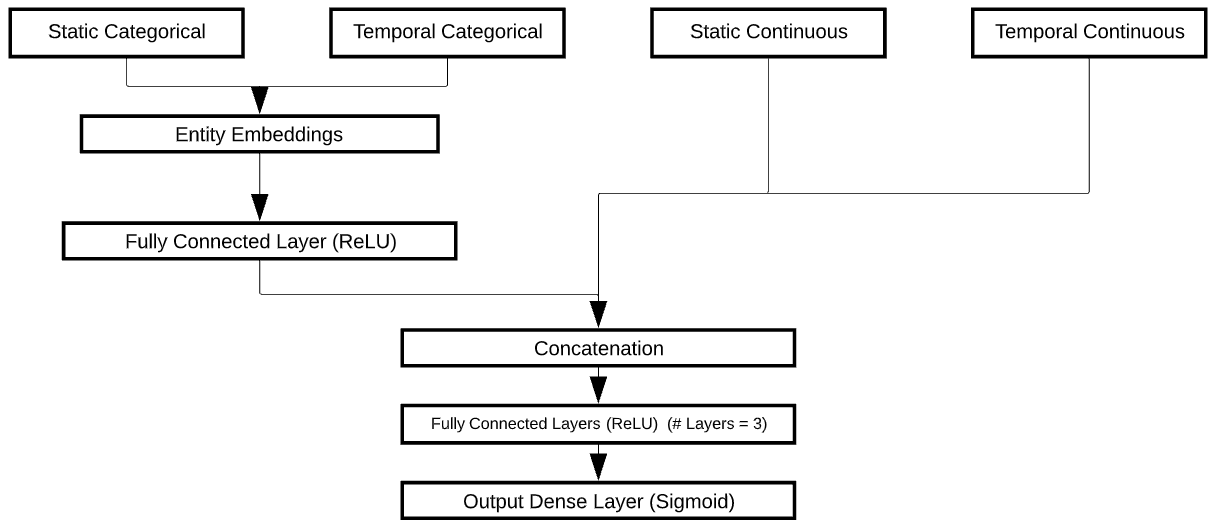
\includegraphics[width=3.3in]{img/MLP.png} 
    \caption{Multi Layer Perceptron (MLP)} 
    \label{fig:MLP} 
  \end{figure}

  \begin{figure}[t]
    \centering 
    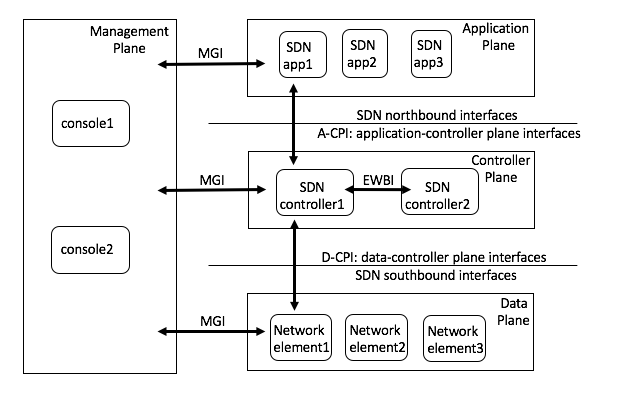
\includegraphics[width=3.3in]{img/LSTM.png} 
    \caption{Long Short Term Memory (LSTM)} 
    \label{fig:LSTM} 
  \end{figure}

  \begin{figure}[t]
    \centering 
    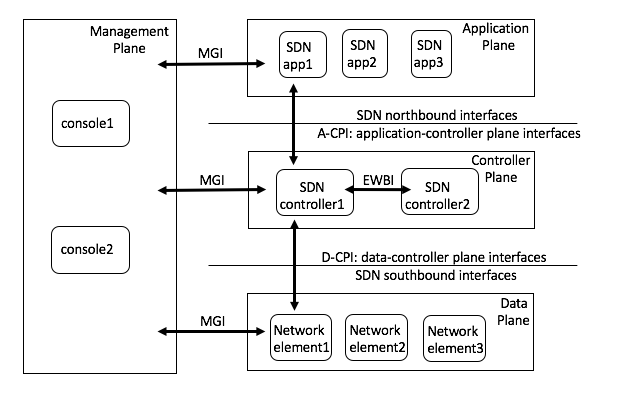
\includegraphics[width=3.3in]{img/CONV1D.png} 
    \caption{Convolution Neural Network 1D (CONV1D)} 
    \label{fig:CONV1D} 
  \end{figure}

  \begin{figure}[t]
    \centering 
    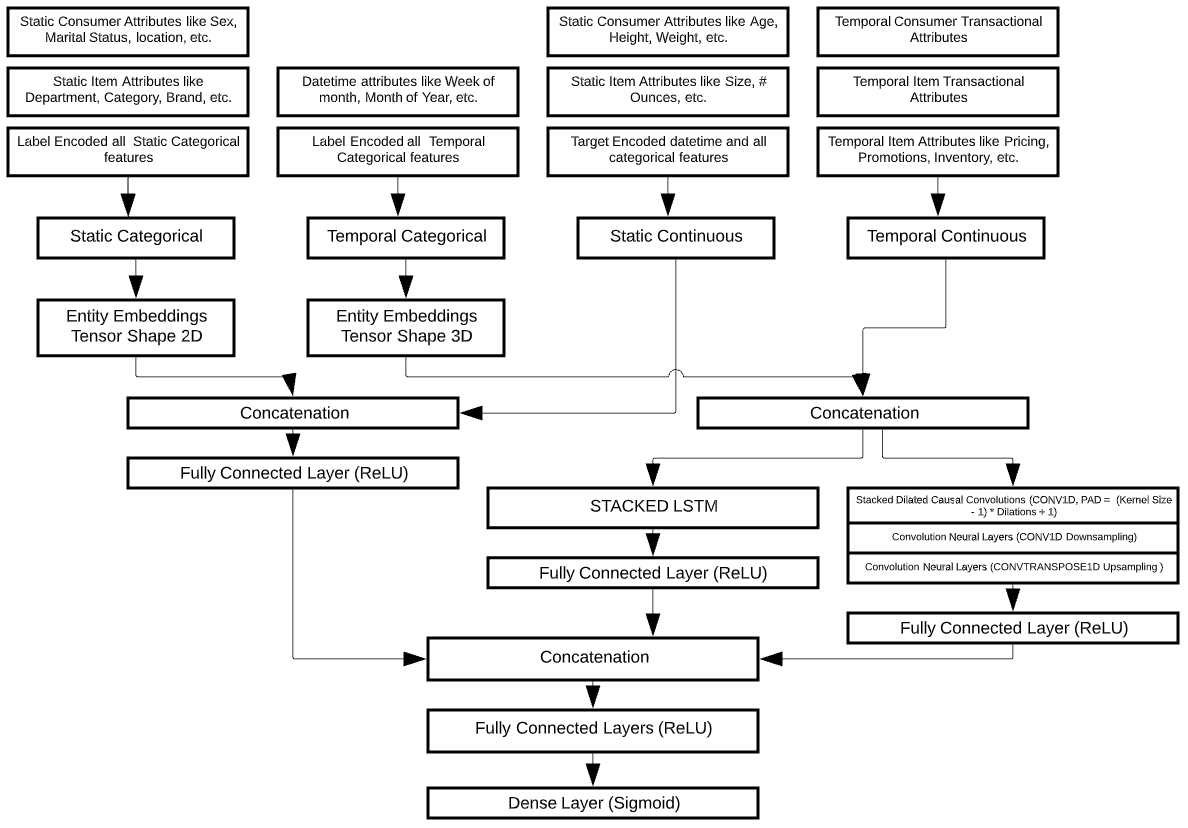
\includegraphics[width=3.3in]{img/CNNLSTM.png} 
    \caption{Convolution Neural Network 1D + Long Short Term Memory (CNNLSTM)} 
    \label{fig:CNNLSTM} 
  \end{figure}

As mentioned in previous section, traditional machine learning models are not suitable choice for solving Equation~\ref{eqn:fx}. 
Hence, we work with machine learning tree based models like Random Forest Gradient Boosted Trees 
to Deep learning models ranging from Multi Layer Perceptron (MLP), Long Short 
Term Memory (LSTM) and Convolution Neural Network (CNN). Architectures of MLP, LSTM, CONV1D and CNNLSTM 
models are shown in Figure~\ref{fig:MLP}, Figure~\ref{fig:LSTM}, Figure~\ref{fig:CONV1D}
and Figure~\ref{fig:CNNLSTM}.

The consumer purchase pattern has huge variation in terms of time of purchase (weekday/weekends), 
cadence of purchase (days to months), purchased item types (dairy/meat/grocery/apparels/etc.)
and brand loyalty (tendency to substitute items). Given such huge variance it becomes imperative 
to cross learn consumer behaviour from like consumer groups. To learn such relationships its very 
important to capture non-linear relationship between target and regressors at the most granular level.
Tree based and Deep learning models are chosen for their ability to model feature interactions even if transient in time, 
so that they capture non-linearity well. Utility of traditional machine learning algorithms like Logistic regression
, SVM and recommender systems are limited given the scale of large retail firms 
(Millions of customers with thousands of products). Such models do not scale well for large sets of data and hyperparameters.

Tree based models and MLP are trained in such a way where lagged values of time varying features are used
to capture temporal dependencies. We use lagged values of temporal features up to last n time steps (n goes till 52 weeks).
Multiple Lagged values as well as Statistical rolling operations like mean, median, quantiles, variance, kurtosis and 
skewness over varying lag periods are used for feature generation. Details around datasets and derived features are explained 
in the following section. This was decided after some preliminary experiments. Hyper-parameters of tree based models are optimized
using Bayesian Hyper-parameter Optimization Technique. LSTM, CONV1D and CNNLSTM models were trained in sequence to sequence 
fashion using entire life-cycle data of a time series (Consumer-Item).

We applied empirical approach to tune the hyperparameters for Deep learning models. All hyperparameter Optimization
was performed over Validation dataset. We list some of the params along with the values we used for Deep learning models.
  \begin{itemize}
    \item {\bf Optimizer Parameters:} RMSProp and Adam were used as different trial configurations. The learning rate 
    was experimentally tuned to 1e-3. We also did weight decay of 1e-5 which helped a bit in model Regularization.
    \item {\bf Scheduler Parameters:} Cyclic and ReduceLROnPlateau Learning rates were used as different trial configurations.
    we used 1e-3 as max lr and 1e-6 as base lr for Cyclical learning rate along with the step size being the function of
    length of train loader. ReduceLROnPlateau was tuned for 1e-6 as min lr.
    \item {\bf SWA:} Stochastic Weight Averaging (SWA) is used to improve generalization across Deep Learning
    models. SWA performs an equal average of the weights traversed by SGD with a modified learning rate schedule. We used 
    1e-3 as SWA learning rate.
    \item {\bf Regularization Parameters:} We also L1 and L2 norm for better generalisation of the models.
  \end{itemize}
Apart from the above parameters we also iterated enough to tune network parameters like number of epochs, batch size, 
number of Fully Connected Layers, number of LSTM layers, convnet parameters (kernel size, dilations, padding)
and embedding sizes for the categorical features. BCELOSS was used a loss function for the backward and forward
passes in Deep Learning setting. Deep learning models are built using deep learning framework
PyTorch, and are trained on GCP instance containing 6 CPUs and a single GPU. scikit-learn is used for Tree
based models like RandomForest and XGBoost. We built a total of 46 models, 9 different param configurations for each of 4 
Deep Learning models and 5 best trials for each of 2 Machine Learning models as shown in table 1.

\begin{table}[t]
\caption{Model Types with Specification}
\vspace{0.1 in}
\centering
\resizebox{6.6in}{!}
{%
\begin{tabular}{c|c|c}
\hline
{\bf Model Type} & {\bf Selected Trials} & {\bf Model Tuning parameters} \\  \hline
MLP	  		&  9 & Optimizer, Scheduler, SWA, Parameter Averaging, Feature Groups, FC Layers \\ \hline
LSTM  		& 9 & Optimizer, Scheduler, SWA, Parameter Averaging, Feature Groups, FC Layers, LSTM Layers  \\ \hline
CONV1D			& 9	& Optimizer, Scheduler, SWA, Parameter Averaging, Feature Groups, FC Layers, Convolution Parameters  \\ \hline
CNNLSTM 		& 9	& Optimizer, Scheduler, SWA, Parameter Averaging, Feature Groups, FC Layers, LSTM, Convolution Parameters  \\ \hline
Xgboost 		& 5	& Learning rate, Tree Depth, Regularization parameters  \\ \hline
RandomForest 		& 5	& Tree Depth, Regularization parameters \\ \hline
\end{tabular}
}
\label{tab:accuracy}
\end{table}

\subsection{Stacked Generalization}
For simplicity and better generalization we adopted non-parameteric approach for stacking.
We used Weighted K Best Stacked Generalization Ensemble for combining the 46 models (candidates) from Table 1. 
Test1 Logloss was used as metric to compute weight for each of the 46 candidates. We set the k to 25 and 
took the Weighted Average of the top 25 candidates based upon Test1 Logloss.

\subsection{F1-Maximization}
Apart from the above parameters we also iterated enough to tune network parameters like number of epochs, batch size, 
number of Fully Connected Layers, number of LSTM layers, convnet parameters (kernel size, dilations, padding)
and embedding sizes for the categorical features.Deep learning models are built using deep learning framework
PyTorch, and are trained on GCP instance containing 6 CPUs and a single GPU. scikit-learn is used for Tree
based models like RandomForest and Xgboost.
